% Note that the a4paper option is mainly intended so that authors in
% countries using A4 can easily print to A4 and see how their papers will
% look in print. Authors are encouraged to use U.S. letter paper when 
% submitting to IEEE. Use the testflow package mentioned above to verify
% correct handling of both paper sizes by the author's LaTeX system.
%
% Also note that the "draftcls" or "draftclsnofoot", not "draft", option
% should be used if it is desired that the figures are to be displayed in
% draft mode.
%
% This paper can be formatted using the peerreviewca
% (instead of conference) mode.
\documentclass[conference, a4paper]{IEEEtran}
% If the IEEEtran.cls has not been installed into the LaTeX system files, 
% manually specify the path to it:
% \documentclass[conference]{../sty/IEEEtran} 


% some very useful LaTeX packages include:
\usepackage{cite}      % Written by Donald Arseneau
                        % V1.6 and later of IEEEtran pre-defines the format
                        % of the cite.sty package \cite{} output to follow
                        % that of IEEE. Loading the cite package will
                        % result in citation numbers being automatically
                        % sorted and properly "ranged". i.e.,
                        % [1], [9], [2], [7], [5], [6]
                        % (without using cite.sty)
                        % will become:
                        % [1], [2], [5]--[7], [9] (using cite.sty)
                        % cite.sty's \cite will automatically add leading
                        % space, if needed. Use cite.sty's noadjust option
                        % (cite.sty V3.8 and later) if you want to turn this
                        % off. cite.sty is already installed on most LaTeX
                        % systems. The latest version can be obtained at:
                        % http://www.ctan.org/tex-archive/macros/latex/contrib/supported/cite/

%\usepackage{graphicx}  % Written by David Carlisle and Sebastian Rahtz
                        % Required if you want graphics, photos, etc.
                        % graphicx.sty is already installed on most LaTeX
                        % systems. The latest version and documentation can
                        % be obtained at:
                        % http://www.ctan.org/tex-archive/macros/latex/required/graphics/
                        % Another good source of documentation is "Using
                        % Imported Graphics in LaTeX2e" by Keith Reckdahl
                        % which can be found as esplatex.ps and epslatex.pdf
                        % at: http://www.ctan.org/tex-archive/info/
% NOTE: for dual use with latex and pdflatex, instead load graphicx like:
\ifx\pdfoutput\undefined
\usepackage[dvipdfm]{graphicx}
\else
\usepackage[pdftex]{graphicx}
\fi

% However, be warned that pdflatex will require graphics to be in PDF
% (not EPS) format and will preclude the use of PostScript based LaTeX
% packages such as psfrag.sty and pstricks.sty. IEEE conferences typically
% allow PDF graphics (and hence pdfLaTeX). However, IEEE journals do not
% (yet) allow image formats other than EPS or TIFF. Therefore, authors of
% journal papers should use traditional LaTeX with EPS graphics.
%
% The path(s) to the graphics files can also be declared: e.g.,
% \graphicspath{{../eps/}{../ps/}}
% if the graphics files are not located in the same directory as the
% .tex file. This can be done in each branch of the conditional above
% (after graphicx is loaded) to handle the EPS and PDF cases separately.
% In this way, full path information will not have to be specified in
% each \includegraphics command.
%
% Note that, when switching from latex to pdflatex and vice-versa, the new
% compiler will have to be run twice to clear some warnings.


%\usepackage{psfrag}    % Written by Craig Barratt, Michael C. Grant,
                        % and David Carlisle
                        % This package allows you to substitute LaTeX
                        % commands for text in imported EPS graphic files.
                        % In this way, LaTeX symbols can be placed into
                        % graphics that have been generated by other
                        % applications. You must use latex->dvips->ps2pdf
                        % workflow (not direct pdf output from pdflatex) if
                        % you wish to use this capability because it works
                        % via some PostScript tricks. Alternatively, the
                        % graphics could be processed as separate files via
                        % psfrag and dvips, then converted to PDF for
                        % inclusion in the main file which uses pdflatex.
                        % Docs are in "The PSfrag System" by Michael C. Grant
                        % and David Carlisle. There is also some information 
                        % about using psfrag in "Using Imported Graphics in
                        % LaTeX2e" by Keith Reckdahl which documents the
                        % graphicx package (see above). The psfrag package
                        % and documentation can be obtained at:
                        % http://www.ctan.org/tex-archive/macros/latex/contrib/supported/psfrag/

\usepackage{subfigure} % Written by Steven Douglas Cochran
                        % This package makes it easy to put subfigures
                        % in your figures. i.e., "figure 1a and 1b"
                        % Docs are in "Using Imported Graphics in LaTeX2e"
                        % by Keith Reckdahl which also documents the graphicx
                        % package (see above). subfigure.sty is already
                        % installed on most LaTeX systems. The latest version
                        % and documentation can be obtained at:
                        % http://www.ctan.org/tex-archive/macros/latex/contrib/supported/subfigure/

\usepackage{url}       % Written by Donald Arseneau
                        % Provides better support for handling and breaking
                        % URLs. url.sty is already installed on most LaTeX
                        % systems. The latest version can be obtained at:
                        % http://www.ctan.org/tex-archive/macros/latex/contrib/other/misc/
                        % Read the url.sty source comments for usage information.

%\usepackage{stfloats}  % Written by Sigitas Tolusis
                        % Gives LaTeX2e the ability to do double column
                        % floats at the bottom of the page as well as the top.
                        % (e.g., "\begin{figure*}[!b]" is not normally
                        % possible in LaTeX2e). This is an invasive package
                        % which rewrites many portions of the LaTeX2e output
                        % routines. It may not work with other packages that
                        % modify the LaTeX2e output routine and/or with other
                        % versions of LaTeX. The latest version and
                        % documentation can be obtained at:
                        % http://www.ctan.org/tex-archive/macros/latex/contrib/supported/sttools/
                        % Documentation is contained in the stfloats.sty
                        % comments as well as in the presfull.pdf file.
                        % Do not use the stfloats baselinefloat ability as
                        % IEEE does not allow \baselineskip to stretch.
                        % Authors submitting work to the IEEE should note
                        % that IEEE rarely uses double column equations and
                        % that authors should try to avoid such use.
                        % Do not be tempted to use the cuted.sty or
                        % midfloat.sty package (by the same author) as IEEE
                        % does not format its papers in such ways.

\usepackage{amsmath}   % From the American Mathematical Society
                        % A popular package that provides many helpful commands
                        % for dealing with mathematics. Note that the AMSmath
                        % package sets \interdisplaylinepenalty to 10000 thus
                        % preventing page breaks from occurring within multiline
                        % equations. Use:
\interdisplaylinepenalty=2500
                        % after loading amsmath to restore such page breaks
                        % as IEEEtran.cls normally does. amsmath.sty is already
                        % installed on most LaTeX systems. The latest version
                        % and documentation can be obtained at:
                        % http://www.ctan.org/tex-archive/macros/latex/required/amslatex/math/



% Other popular packages for formatting tables and equations include:

%\usepackage{array}
% Frank Mittelbach's and David Carlisle's array.sty which improves the
% LaTeX2e array and tabular environments to provide better appearances and
% additional user controls. array.sty is already installed on most systems.
% The latest version and documentation can be obtained at:
% http://www.ctan.org/tex-archive/macros/latex/required/tools/

% Mark Wooding's extremely powerful MDW tools, especially mdwmath.sty and
% mdwtab.sty which are used to format equations and tables, respectively.
% The MDWtools set is already installed on most LaTeX systems. The lastest
% version and documentation is available at:
% http://www.ctan.org/tex-archive/macros/latex/contrib/supported/mdwtools/


% V1.6 of IEEEtran contains the IEEEeqnarray family of commands that can
% be used to generate multiline equations as well as matrices, tables, etc.


% Also of notable interest:

% Scott Pakin's eqparbox package for creating (automatically sized) equal
% width boxes. Available:
% http://www.ctan.org/tex-archive/macros/latex/contrib/supported/eqparbox/



% Notes on hyperref:
% IEEEtran.cls attempts to be compliant with the hyperref package, written
% by Heiko Oberdiek and Sebastian Rahtz, which provides hyperlinks within
% a document as well as an index for PDF files (produced via pdflatex).
% However, it is a tad difficult to properly interface LaTeX classes and
% packages with this (necessarily) complex and invasive package. It is
% recommended that hyperref not be used for work that is to be submitted
% to the IEEE. Users who wish to use hyperref *must* ensure that their
% hyperref version is 6.72u or later *and* IEEEtran.cls is version 1.6b 
% or later. The latest version of hyperref can be obtained at:
%
% http://www.ctan.org/tex-archive/macros/latex/contrib/supported/hyperref/
%
% Also, be aware that cite.sty (as of version 3.9, 11/2001) and hyperref.sty
% (as of version 6.72t, 2002/07/25) do not work optimally together.
% To mediate the differences between these two packages, IEEEtran.cls, as
% of v1.6b, predefines a command that fools hyperref into thinking that
% the natbib package is being used - causing it not to modify the existing
% citation commands, and allowing cite.sty to operate as normal. However,
% as a result, citation numbers will not be hyperlinked. Another side effect
% of this approach is that the natbib.sty package will not properly load
% under IEEEtran.cls. However, current versions of natbib are not capable
% of compressing and sorting citation numbers in IEEE's style - so this
% should not be an issue. If, for some strange reason, the user wants to
% load natbib.sty under IEEEtran.cls, the following code must be placed
% before natbib.sty can be loaded:
%
% \makeatletter
% \let\NAT@parse\undefined
% \makeatother
%
% Hyperref should be loaded differently depending on whether pdflatex
% or traditional latex is being used:
%
\ifx\pdfoutput\undefined
\usepackage[hypertex,dvipdfm]{hyperref}
\else
\usepackage[pdftex,hypertexnames=false,pdfstartview=FitH]{hyperref}
\fi
%
% Pdflatex produces superior hyperref results and is the recommended
% compiler for such use.



% *** Do not adjust lengths that control margins, column widths, etc. ***
% *** Do not use packages that alter fonts (such as pslatex).         ***
% There should be no need to do such things with IEEEtran.cls V1.6 and later.


% correct bad hyphenation here
\hyphenation{op-tical net-works semi-conduc-tor IEEEtran}

%\usepackage[left=25mm,right=25mm,top=25mm,bottom=25mm,columnsep=9mm]{geometry}
\usepackage[thinspace,thinqspace]{SIunits}
\usepackage{mathrsfs}
\usepackage{multirow}
% \IEEEoverridecommandlockouts
%\usepackage{mt11p}
\begin{document}

% paper title
\title{Weighted Laguerre Polynomials and its Applications in Transient RCS
Analysis}

% author names and affiliations
% use a multiple column layout for up to three different
% affiliations
% \author{\authorblockN{Michael Shell}
% \authorblockA{School of Electrical and\\Computer Engineering\\
% Georgia Institute of Technology\\
% Atlanta, Georgia 30332--0250\\
% Email: mshell@ece.gatech.edu}
% \and
% \authorblockN{Homer Simpson}
% \authorblockA{Twentieth Century Fox\\
% Springfield, USA\\
% Email: homer@thesimpsons.com}
% \and
% \authorblockN{James Kirk\\ and Montgomery Scott}
% \authorblockA{Starfleet Academy\\
% San Francisco, California 96678-2391\\
% Telephone: (800) 555--1212\\
% Fax: (888) 555--1212}}


% avoiding spaces at the end of the author lines is not a problem with
% conference papers because we don't use \thanks or \IEEEmembership


% for over three affiliations, or if they all won't fit within the width
% of the page, use this alternative format:
% 
\author{\authorblockN{Wenfeng Cai, Xueguan Liu, Huiping Guo and Honglong Cao }
\authorblockA{School of Electronics and Information Engineering\\
Soochow University, Suzhou, Jiangsu, P. R. China\hspace{1em}215021\\
Email: caiwenfeng@suda.edu.cn}
}



% use only for invited papers
%\specialpapernotice{(Invited Paper)}

% make the title area
\maketitle

\begin{abstract}
Weighted Laguerre polynomial is a set of self-contained orthogonal
causal functions. In this paper, the properties of weighted Laguerre
polynomials are summarized. As a set of temporal basis functions, the
influence and choice of the time scaling factor are discussed in detail.
And then the choise principle for the time scaling factor is obtained.The
application of weighted Laguerre polynomials, which are  the temporal
basis of transient scattering analysis for arbitrary shaped structures,
is illustrated for transient RCS calculation. The examples show that the choice
principle proposed here is effective.
\end{abstract}
% \vspace{1.34ex}
%\begin{keywords}
%\end{keywords}

% For peer review papers, you can put extra information on the cover
% page as needed:
% \begin{center} \bfseries EDICS Category: 3-BBND \end{center}
%
% for peerreview papers, inserts a page break and creates the second title.
% Will be ignored for other modes.
\IEEEpeerreviewmaketitle



\section{Introduction}
% no \PARstart
Recently, along with the development of new solutions, the wide-band response of
electromagnetic scattering has received considerable attention
\cite{kashyap:stabilizing:1998,hujinlin:temporal:2001,jung:cfie:2002,jizhong:solving:2006}.
Researches
on time-domain integral equation have more remarkable development. T. K.
Sarkar {\em et al.} present a marching on in order method, which
reduces the late-time instability of marching on in time (MOT) related
methods \cite{jizhong:solving:2006,jung:accurate:2002,jung:analysis:2004,jung:time:2003}. In these algorithms the time-domain integral equations
are expressed in terms of weighted Laguerre polynomials with a time
scaling factor. The scaling parameters are chosen in above references
without given a general principle for choosing an optimal one. In this
paper, based on the analysis to the characteristics of weighted Laguerre
polynomials, the effects of the time scaling factor are discussed and the
principle of choosing an optimal one is proposed. Further, transient scattering analysis for arbitrary shaped structures is studied using the 
weighted Laguerre polynomials as temporal basis. The calculation examples show that the choice
principle for time scaling factor proposed here is effective.
 
% Reminder: the "draftcls" or "draftclsnofoot", not "draft", class option
% should be used if it is desired that the figures are to be displayed while
% in draft mode.

% An example of a floating figure using the graphicx package.
% Note that \label must occur AFTER (or within) \caption.
% For figures, \caption should occur after the \includegraphics.
%
%\begin{figure}
%\centering
%\includegraphics[width=2.5in]{myfigure}
% where an .eps filename suffix will be assumed under latex, 
% and a .pdf suffix will be assumed for pdflatex
%\caption{Simulation Results}
%\label{fig_sim}
%\end{figure}


% An example of a double column floating figure using two subfigures.
%(The subfigure.sty package must be loaded for this to work.)
% The subfigure \label commands are set within each subfigure command, the
% \label for the overall fgure must come after \caption.
% \hfil must be used as a separator to get equal spacing
%
%\begin{figure*}
%\centerline{\subfigure[Case I]{\includegraphics[width=2.5in]{subfigcase1}
% where an .eps filename suffix will be assumed under latex, 
% and a .pdf suffix will be assumed for pdflatex
%\label{fig_first_case}}
%\hfil
%\subfigure[Case II]{\includegraphics[width=2.5in]{subfigcase2}
% where an .eps filename suffix will be assumed under latex, 
% and a .pdf suffix will be assumed for pdflatex
%\label{fig_second_case}}}
%\caption{Simulation results}
%\label{fig_sim}
%\end{figure*}



% An example of a floating table. Note that, for IEEE style tables, the 
% \caption command should come BEFORE the table. Table text will default to
% \footnotesize as IEEE normally uses this smaller font for tables.
% The \label must come after \caption as always.
%
%\begin{table}
%% increase table row spacing, adjust to taste
%\renewcommand{\arraystretch}{1.3}
%\caption{An Example of a Table}
%\label{table_example}
%\begin{center}
%% Some packages, such as MDW tools, offer better commands for making tables
%% than the plain LaTeX2e tabular which is used here.
%\begin{tabular}{|c||c|}
%\hline
%One & Two\\
%\hline
%Three & Four\\
%\hline
%\end{tabular}
%\end{center}
%\end{table}

\section{The Characteristic Properties of the Weighted Laguerre
Polynomials}

The normalized order $k$ Laguerre polynomial can be expressed as
\begin{equation}
L_k(t)=\frac{\mathrm{e}^t}{k!}\frac{\mathrm{d}^k}{\mathrm{d}t^k}(t^k\mathrm{e}^{-t}),\;
\text{for $k\ge 0,\:t\ge 0$}.
\end{equation}
These polynomials satisfy a recursive relationship given by
\begin{equation}
\begin{split}
L_0(t)&=1 \\
L_1(t)&=1-t \\
L_k(t)&=\frac{1}{k}\left [ (2k-1-t)L_{k-1}(t)\right . \\
 &\quad \left . -(k-1)L_{k-2}(t)\right ]
\;\;\;\;\text{for $k\ge 2$.}
\end{split}
\end{equation}
They are orthogonal with respect to the weighted function
$\mathrm{e}^{-t}$, given by
\begin{equation}
\int _{0}^{\infty}\mathrm{e}^{-t}L_i(t)L_k(t)\mathrm{d}t=\delta _{ik},
\end{equation}
where $\delta _{ik}$ is a Kronecker delta for $i=k$ and zero otherwise.
Therefore, an orthonormal set of basis functions at $[0,\:\infty)$ can be derived through
the representation
\begin{equation}
\phi _k(t)=\mathrm{e}^{-t/2}L_k(t).
\end{equation}
Using these basis functions, any arbitrary causal signal $e_n(t)$ can be
expanded as
\begin{equation}
e_n(t)=\sum _{k=0}^{\infty}c_{n,k}\phi _k(st),
\end{equation}
where $s>0$ is a time scaling factor. By controlling the time scaling
factor, the support provided by the expansion can be increased or
decreased.

The weighted Laguerre polynomials mentioned here have the following
characteristic properties.
\begin{enumerate}
\item derivative \cite{jung:time:2003}: $L_k'(y)=L_k(y)-(k+1)L_k(y)$. The first and second
derivatives of $e_n(t)$ with respect to time $t$ can be expressed as
\begin{equation}
\begin{split}
\dot{e}_n(t)&=s\sum _{k=0}^{\infty}\left [\frac{1}{2}c_{n,k}+\sum
_{i=0}^{k-1}c_{n,i}\right ]\phi _k(st) \\
\ddot{e}_n(t)&=s^2\sum _{k=0}^{\infty}\left [\frac{1}{4}c_{n,k}+\sum
_{i=0}^{k-1}c_{n,i}\right ]\phi _k(st).
\end{split}
\end{equation}
\item integration \cite{gradshteyn:table:1980}:
\begin{equation}
\begin{split}
I_{ik}(st_0)&=\int
_0^{\infty}\phi_i(st)\phi_k(st-st_0)\mathrm{d}(st) \\
&=\begin{cases}\mathrm{e}^{-st_0/2}[L_{i-k}(st_0)-L_{i-k-1}(st_0)]&k<i\\
    \mathrm{e}^{-st_0/2}&k=i\\
    0&k>i\end{cases}
\end{split}
\end{equation}
\item limit: 
\begin{equation}
\lim _{y\rightarrow 0}\frac{\phi_k(y)-1}{y}=-(k+\frac{1}{2}).
\end{equation}
\end{enumerate}

\section{Choice of the Scaling Factor $s$}

The Fourier transform of order $k$ weighted Laguerre polynomial is
\begin{equation}
\begin{split}
\Phi_k(\mathrm{j}\omega)&=\frac{(-1/2+\mathrm{j}\omega)^k}{(1/2+\mathrm{j}\omega)^{k+1}}\\
\lvert{\Phi_k(\mathrm{j}\omega)}\rvert&=\frac{2}{\sqrt{1+4\omega^2}},
\end{split}
\end{equation}
which is shown in Fig.~\ref{fig1}. Its $\unit{-20}{\deci\bel}$
bandwidth is about $\unit{0.8}{\hertz}$. As the basis functions for a
$\unit{}{\mega\hertz}\sim\unit{}{\giga\hertz}$ signal, this scale is very
small. In order to use the above basis functions in an appropriate
fashion, one should transform the interval using an appropriate scaling 
factor $s$. Since the Fourier transform obeys a similarity theorem,
changing temporal scale inversely affects frequency and amplitude, that is,
\begin{equation}
\mathscr{F}[\phi_k(st)]=\frac{1}{s}\Phi_k(\frac{\mathrm{j}\omega}{s}).
\end{equation}
\begin{figure}
    \centering
    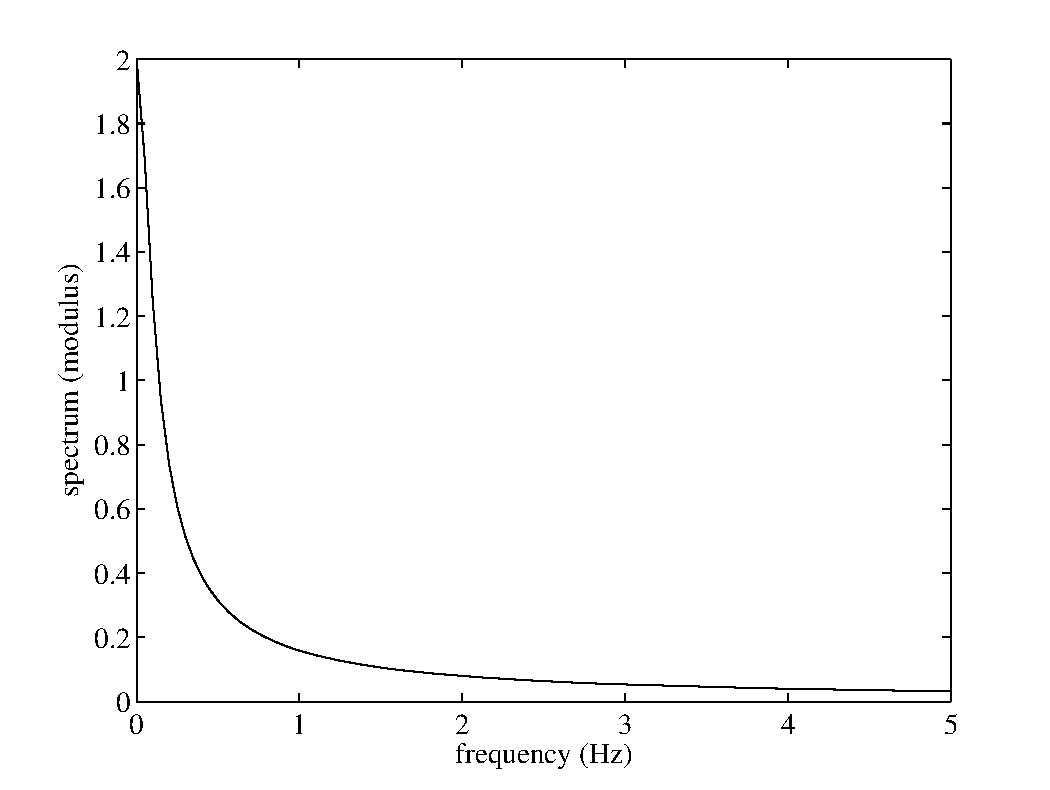
\includegraphics[scale=0.48]{lagu.pdf}
    \caption{The Fourier spectrum of weighted Laguerre polynomials.}
    \label{fig1}
\end{figure}

Let's take a look at the principles to choose an optimal time scaling factor
$s$. Consider an arbitrary causal signal $f(t)$ with time duration of $T_f$
and approximately band limited on $B$, which can be expressed by the
orthogonal weighted Laguerre polynomials as
\begin{equation}
f(t)=\sum_{k=0}^{N}a_k\phi_k(st).
\end{equation}
Theoretically there should be $N\rightarrow\infty$. Since the signal that
we are interested in characterizing is practically bandlimited up to
$B$, Ref.~\cite{jung:time:2003} proposes the minimum number of temporal basis
functions is $2BT_f+1$. If the number of basis functions is less than
this minimum number, the results will be unacceptable.

It's important to search for a better value of time scaling factor $s$ to
expand an causal signal correctly. If $s$ is too small, the spectrum of
basis functions will not cover the one of original signal; and if $s$ is
too big, the original signal can not either be expressed by the weighted
Laguerre polynomials. Here shows the effect of $s$ when a Gaussian pulse
is expanded with the mentioned basis functions.

A Gaussian pulse is mathematically represented by
\begin{equation}
f(t)=\mathrm{e}^{-\gamma^2}
\end{equation}
where $\gamma=(4/T)(ct-ct_0)$, $c$ is the velocity of light in the air.
We use $T=4$ and $ct_0=10$. Both of these quantities are defined in
light meters (lm), which is the time taken by light to traverse
\unit{1}{\meter}. The $\unit{-40}{\deci\bel}$ bandwidth $B$ of the pulse
is approximately $\unit{750}{\mega\hertz}$, $T_f\approx 20/c$. We now
compute the error between the constructed signal with basis functions
and the original signal as follows:
\begin{equation}
\epsilon(s)=\sqrt{\int_0^\infty\left | f(t)-\sum_{k=0}^N
a_k\phi_k(st)\right | ^2\mathrm{d}t}.\label{error-eq}
\end{equation}
Fig.~\ref{error} plot the error given by (\ref{error-eq}) as a function of
the time scaling factor $s$. As can be seen the appropriate $s$ can
give more accurate results. In our example, the optimal $s=nB,\;\;(n=2\sim 5)$.
\begin{figure}
    \centering
    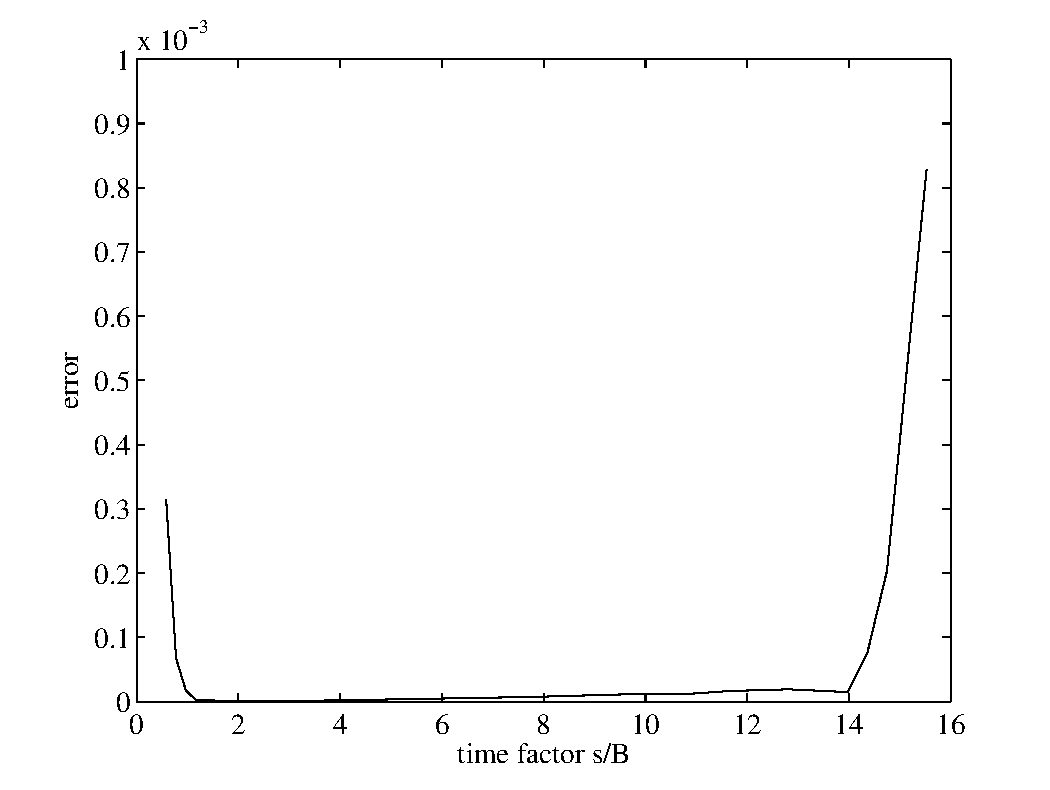
\includegraphics[scale=.48]{error.pdf}
    \caption{The error along with different $s$.}
    \label{error}
\end{figure}

\section{The Application of Weighted Laguerre Polynomials in Transient
RCS Analysis}
The scattering from a conducting sphere is simulated with the 
marching-on-in-order method \cite{jizhong:solving:2006}, in which the integral equation is
solved by expressing the transient bebaviors in terms of the Laguerre
functions. The sphere is with a spatial discretization of 909 common
edges and has a radius of \unit{0.45}{\meter}. The scattering from this
sphere have been simulated when the excitation is the Gaussian pluse
with $T=99.7(\mathrm{lm})$, $ct_0=100.5(\mathrm{lm})$.
Fig.~\ref{scatter} shows the backward scattered farfield from the sphere
when the scaling factor $s$ are $0.40c$, $0.80c$, $0.16c$, $1.60c$,
respectively, where $0.40c$ and $0.80c$ are in the range obtained from
the above principles for searching optimal $s$ scaling factor, $0.16c$ and
$1.60c$ is out of that range. The results gotten with $s=0.40c$ and $s=0.80c$ agree well
with the theoretical results for the same object. The other two curves
then is not very accurate. 
\begin{figure}
    \centering
    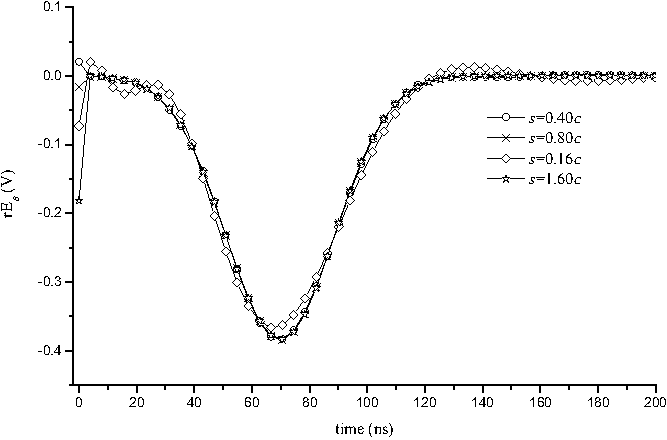
\includegraphics[scale=.75]{scatter.pdf}
    \caption{Backward farfield of a sphere excited by a Gaussian pulse
    expressed in terms of the Laguerre functions with different time
    scaling factor $s$.}
    \label{scatter}
\end{figure}

\section{Conclusion}

It's worthy to research thoroughly the properties of weighted Laguerre
polynomials for transient electromagnetic scattering problems. In this
paper, the time domain characteristics of weighted Laguerre polynomials are
studied. The influence of the time scaling factor and its choice
principles are also discussed,
which establish the basis of transient
electromagnetic scattering analysis and should be further researched.

% conference papers do not normally have an appendix

% use section* for acknowledgement
% \section*{Acknowledgment}
% optional entry into table of contents (if used)
%\addcontentsline{toc}{section}{Acknowledgment}
% The authors would like to thank...

% trigger a \newpage just before the given reference
% number - used to balance the columns on the last page
% adjust value as needed - may need to be readjusted if
% the document is modified later
% \IEEEtriggeratref{3}
% The "triggered" command can be changed if desired:
%\IEEEtriggercmd{\enlargethispage{-5in}}
\enlargethispage{-12.5cm}
%\nocite{mittr73}
% references section
% NOTE: BibTeX documentation can be easily obtained at:
% http://www.ctan.org/tex-archive/biblio/bibtex/contrib/doc/

% can use a bibliography generated by BibTeX as a .bbl file
% standard IEEE bibliography style from:
% http://www.ctan.org/tex-archive/macros/latex/contrib/supported/IEEEtran/bibtex
\bibliographystyle{IEEEtran}
% argument is your BibTeX string definitions and bibliography database(s)
\bibliography{IEEEabrv,mybib}
%
% <OR> manually copy in the resultant .bbl file
% set second argument of \begin to the number of references
% (used to reserve space for the reference number labels box)
% that's all folks
\end{document}


